\chapter{Marketing}
\begin{flushleft}
    Marketing befasst sich damit ein Produkt unter Menschen zu bringen.
    Dabei soll das Image des Unternehmens erhalten werden.
    Setzt ein Unternehmen Marketing richtig ein, gewinnt und bindet es Kunden.
\end{flushleft}

\section{Marketing-Mix}
\begin{flushleft}
    Der Marketing-Mix besteht aus verschiedenen Marketinginstrumenten, er befasst 
    sich hauptsächlich mit der Umsetzung dieser Instrumente durch Marketingstrategien. \\
    Gänige Marketinginstrumente sind die Produktpolitik, Preispolitik, Vertriebspolitik
    und Kommunikationspolitik. Diese werden auch die vier P's genannt
    (product, price, place, promotion).
\end{flushleft}

\subsection{Produktpolitik}
\subsubsection{Definition}
\begin{flushleft}
    Die Produktpolitik trifft alle Entscheidungen, die das Produkt eines Unternehmens betreffen.
    Beispielsweise entscheidet die Produktpolitik über die Qualität, Funktionalität und das Design
    des Produktes.
\end{flushleft}

\subsubsection{Maßnahmen}
\begin{flushleft}
    Die Produktpolitik orientiert sich an dem \hyperref[subsec:Produktlebenszyklus]{Produktlebenszyklus}
    eines Produktes. Abhängig von der Phase des Produktlebenszyklus nutzt die Produktpolitik eine dieser
    Maßnahmen:
    \begin{enumerate}
        \item {
            \textbf{Produktinnovation} \\
            Das Unternehmen entwickelt neue Produkte um Marktanteile zu bekommen.
        }
        \item {
            \textbf{Produktvariation} \\
            Bestehende Produkte werden weiterentwickelt (``variiert'').
        }
        \item {
            \textbf{Produktelemination} \\
            Produkte, die keine Gewinne mehr abwerfen werden aus dem Portfolio gestrichen.
        }
    \end{enumerate}
\end{flushleft}

\subsection{Preispolitik}
\subsubsection{Preisbildung}
\begin{flushleft}
    Die Preispolitik bestimmt den Preis eines Produktes.
    Dabei kann sich die Preispolitik an verschiedenen Faktoren orientieren.
    Es gibt daher die kosten-, nachfrage- und konkurrenzorientierte Preisbildung.
    \begin{enumerate}
        \item {
            \textbf{Kostenorientierte Preisbildung} \\
            Diese Art der Preisbildung basiert auf der Kostenstruktur des Unternehmens.
            Kosten werden in fixe, variable, Stück-, Gesamt-, Einzel- und Gemeinkosten unterteilt.
            Wichtig sind hierbei die \textbf{Break-even-Point-Analyse} und die \textbf{Preisuntergrenzen}.
            Bei der Break-even-Point-Analyse wird ermittelt ab welcher Absatzmenge Gewinn gemacht wird.
            Die Preisuntergrenzen werden in verschiedene Arten unterschieden:
            \begin{enumerate}
                \item {
                    langfristige Preisuntergrenze
                    \[PU=k_v+k_f\]
                }
                \item {
                    kurzfristige Preisuntergrenze
                    \[PU=k_v\]
                }
                \item {
                    liquiditätsorientierte Preisuntergrenze (ausgabewirksame Fixkosten sind z.B. Löhne, Gehälter und Mieten)
                    \[PU=k_v+\text{ausgabewirksame}~k_f\]
                }
            \end{enumerate}
        }
        \item {
            \textbf{Nachfrageorientierte Preisbildung} \\
            Die nachfrageorientierte Preisbildung orientiert sich an dem Preis, den die Käufer bereit sind zu zahlen.
            Sie nutzt hauptsächlich diese beiden Strategien:
            \begin{enumerate}
                \item {
                    \textbf{Conjoint-Measurement} \\
                    \begin{enumerate}
                        \item Findet heraus welche Produkteigenschaften für den Kunden wichtig sind
                        \item Preis kann durch die Kostenstruktur der einzelnen, bevorzugten Eigenschaften gebildet werden
                    \end{enumerate}
                }
                \item {
                    \textbf{Preisdifferenzierung} \\
                    \begin{enumerate}
                        \item Unterschiedliche Preise für verschiedene Zielgruppen
                    \end{enumerate}
                }
            \end{enumerate}
        }
        \item {
            \textbf{Konkurrenzorientierte Preisbildung} \\
            Der Preis orientiert sich am Markt, also an der Konkurrenz.
            Um sich am Markt orientieren zu können muss herausgefunden werden in welchem Markt man sich befindet.
            Man unterscheidet zwischen vollkommenen und unvollkommenen Märkten, ein monopolistischer Markt ist ein unvollkommener Markt:
            \begin{enumerate}
                \item {
                    \textbf{monopolistischer Markt} \\
                    Der Preis ist das Maximum der Gewinnfunktion;
                    das Unternehmen hat ein Marktmonopol und möchte den Gewinn maximieren.
                }
                \item {
                    \textbf{vollkommener Markt} \\
                    Ein vollkommener Markt liegt vor wenn all diese Bedingungen erfüllt sind:
                    \begin{enumerate}
                        \item Viele kleine Anbieter und Nachfrager mit kleinem Marktanteil; kein Unternehmen hat eine relevante Marktmacht
                        \item Die Güter aller Anbieter sind gleich
                        \item Nachfrager haben keine sachlichen, räumlichen, zeitlichen und persönlichen Vorlieben
                        \item Anbieter und Nachfrage haben alle marktrelevanten Informationen
                        \item Jeder darf anbieten oder nachfragen
                        \item Der Markt reagiert sofort
                        \item Marktteilnehmer sind rational
                    \end{enumerate}
                    Im vollkommenen Markt liegt ein Gleichgewichtspreis vor. Der Gleichgewichtspreis ist der Schnittpunkt zwischen der Angebots- und der Nachfragekurve.
                    Ein vollkommener Markt ist ein rein theoretisches Modell.
                }
                \item {
                    \textbf{unvollkommener Markt} \\
                    Ein Markt ist unvollkommen, wenn eine Bedingung des vollkommenen Marktes nicht erfüllt ist.
                    Hier wird wieder in verschiedene Märkte unterschieden:
                    \begin{enumerate}
                        \item {
                            \textbf{oligopolistischer Markt} \\
                            Ein oligopolistischer Markt hat viele Nachfrager aber wenig Anbieter.
                        }
                        \item {
                            \textbf{polypolistischer Markt} \\
                            Polypolistische Märkte verfügen über viele Nachfrager und viele Anbieter.
                        }
                    \end{enumerate}
                }
            \end{enumerate} 
        }
    \end{enumerate}
\end{flushleft}

\subsubsection{Preisstrategien}
\begin{flushleft}
    In der Praxis werden oft auch Preisstrategien genutzt um den Gewinn zu maximieren:
    \begin{enumerate}
        \item {
            \textbf{Hochpreispolitik (Premiumpolitik)} \\
            Der Preis wird im Vergleich zur Konkurrenz hoch angesetzt, das funktioniert indem mit einer höheren Qualität geworben wird.
            Das Ziel sind also keine besonders großen Absatzmengen sondern hohe Preise mit guter Qualität bei niedrigeren Absatzmengen.
        }
        \item {
            \textbf{Niedrigpreispolitik (Promotionspolitik)} \\
            Der Preis wird im Vergleich zur Konkurrenz niedrig angesetzt, das funktioniert indem mit diesem niedrigeren Preis geworben wird.
            Hier sind hohe Absatzmengen bei einem niedrigen Gewinn pro Stück das Ziel.
        }
        \item {
            \textbf{Marktabschöpfungspolitik (Skimmingpolitik)} \\
            Zur Einführung eines neuen Produktes wird der Preis dieses Produktes hoch angesetzt, mit der Zeit wird der Preis jedoch verringert,
            da Konkurrenten Substitutionsgüter anbieten.
        }
        \item {
            \textbf{Marktdurchdringungspolitik (Penetrationspolitik)} \\
            Bei dieser Strategie ist das Ziel die Kunden an ein Produkt zu binden.
            Das funktioniert indem ein Produkt anfangs zu einem niedrigen Preis angeboten wird und dieser Preis dann nach und nach
            angehoben wird. So wird das Produkt zur Einführung oft verkauft und die gewonnenen Kunden sind meist
            bereit das Produkt auch nach einer Preiserhöhung erneut zu kaufen.
        }
    \end{enumerate}
\end{flushleft}

\subsection{Vertriebspolitik}
\subsection{Kommunikationspolitik}

\section{Strategische Analysen}
\subsection{SWOT-Analyse}
\pagebreak

\subsection{Produktlebenszyklus}\label{subsec:Produktlebenszyklus}
\begin{flushleft}
    Die Idee hinter dem Produktlebenszyklus ist, dass jedes Produkt einen Lebenszyklus durchläuft.
    Dieser Lebenszyklus wird in fünf verschiedene Phasen eingeteilt.
    Basierend auf der momentanen Phase eines Produktes kann dann abgeschätzt werden, was
    mit diesem Produkt passieren sollte (eliminieren, \dots).
\end{flushleft}

\begin{center}
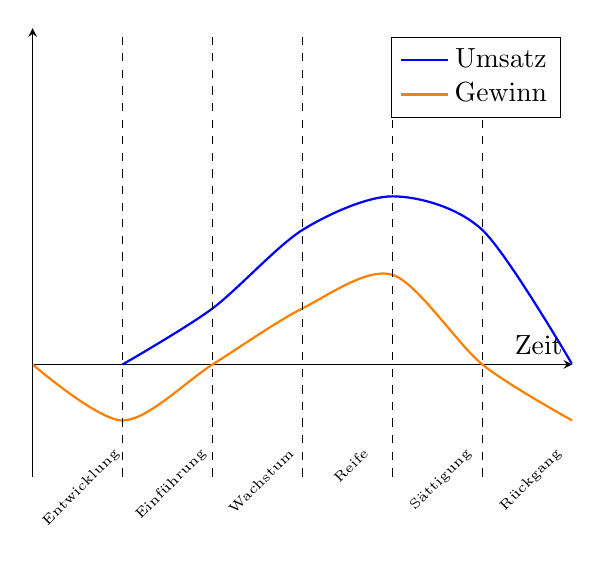
\begin{tikzpicture}
\begin{axis}[
    axis lines=middle,
    xtick=\empty,
    ytick=\empty,
    extra x ticks={1,2,3,4,5,6},
    extra x tick style={major tick length=0pt,yshift=-25pt,xshift=-15pt,opacity=1,grid=none,xticklabel style={font=\tiny ,rotate=45}},
    extra x tick labels={
        Entwicklung,Einführung,Wachstum,Reife,Sättigung,Rückgang
    },
    ymax=3,
    ymin=-1,
    xlabel={Zeit},
    ylabel={\euro}
]
\addplot[blue,smooth,thick] coordinates {
    (1,0) (2,0.5) (3,1.2) (4,1.5) (5,1.2) (6,0)
};
\addlegendentry{Umsatz}
\addplot[orange,smooth,thick] coordinates {
    (0,0) (1,-0.5) (2,0) (3,0.5) (4,0.8) (5,0) (6,-0.5)
};
\addlegendentry{Gewinn}
\draw[color=black, dashed] (axis cs:1, -1) -- (axis cs:1, 3);
\draw[color=black, dashed] (axis cs:2, -1) -- (axis cs:2, 3);
\draw[color=black, dashed] (axis cs:3, -1) -- (axis cs:3, 3);
\draw[color=black, dashed] (axis cs:4, -1) -- (axis cs:4, 3);
\draw[color=black, dashed] (axis cs:5, -1) -- (axis cs:5, 3);
\end{axis}
\end{tikzpicture}
\end{center}

\begin{flushleft}
    Jede Phase verfügt über verschiedene Merkmale.
\end{flushleft}
\begin{center}
\begin{tabular}{|l|p{8cm}|}
    \hline
    \textbf{Phase} & \textbf{Merkmale} \\
    \hline
    Entwicklung & Das Produkt befindet sich noch in der Entwicklung und deshalb noch nicht auf dem Markt. Es hat bisher nur Kosten verursacht. \\
    \hline
    Einführung & Das Produkt wird in den Markt eingeführt. Dabei entstehen jedoch hohe Kosten durch Werbung. Zum Ende dieser Phase sollte das Produkt die Kosten decken können. \\
    \hline
    Wachstum & In der Wachstumsphase steigt der Umsatz des Produktes stark an. Der Markt ist jedoch noch stark umkämpft, deshalb bleiben hohe Werbekosten. \\
    \hline
    Reife & Die Reifephase zeigt hohe Gewinne während der Umsatz weniger steigt als in der Wachstumsphase. Nach der Reifephase fallen Gewinn und Umsatz. \\
    \hline
    Sättigung & In der Sättigungsphase fallen Umsatz und Gewinn, zum Ende dieser Phase wird meist kein Gewinn mehr erzielt. \\
    \hline
    Rückgang & In der Phase des Rückgangs oder der Degeneration macht das Produkt Verlust. Es ist die letzte Phase des Produktlebenszyklus und damit das Ende des Produktes. \\
    \hline
\end{tabular}
\end{center}

\subsection{Portfolioanalyse (BCG-Matrix)}
\begin{flushleft}
    Die Portfolioanalyse ist eine Analysestrategie, die eine übersichtliche Darstellung des gesamten
    Portfolio erlaubt. Bei einer Portfolioanalyse wird eine Vierfeldmatrix erstellt, diese Matrix wird auch BCG-Matrix
    genannt, da sie durch die Boston Consulting Group bekannt wurde. Die vier Felder stellen die vier Produktlebensphasen dar.
\end{flushleft}
\begin{center}
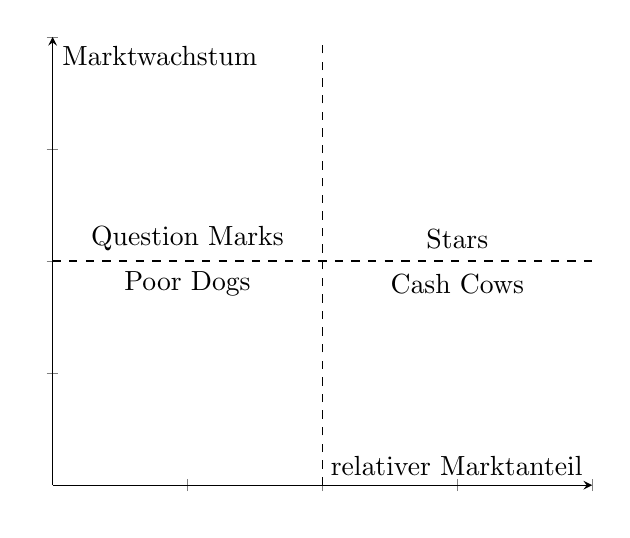
\begin{tikzpicture}
\begin{axis}[
    axis lines=middle,
    xlabel={relativer Marktanteil},
    ylabel={Marktwachstum},
    xmax=2,
    xmin=0,
    ymax=2,
    ymin=0,
    xticklabel=\empty,
    yticklabel=\empty
]
\addplot[draw=none] coordinates {
    (0,0)
};
\draw[color=black, dashed] (axis cs:0, 1) -- (axis cs:2, 1);
\draw[color=black, dashed] (axis cs:1, 0) -- (axis cs:1, 2);
\draw (axis cs:0.5,1.1) node {Question Marks};
\draw (axis cs:1.5,1.1) node {Stars};
\draw (axis cs:0.5,0.9) node {Poor Dogs};
\draw (axis cs:1.5,0.9) node {Cash Cows};
\end{axis}
\end{tikzpicture}
\end{center}

\begin{flushleft}
    So wie bei dem Produktlebenszyklus gibt es hier verschiedene Merkmale für die Produktlebensphasen.
\end{flushleft}
\begin{center}
\begin{tabular}{|l|p{8cm}|}
    \hline
    \textbf{Phase} & \textbf{Merkmale} \\
    \hline
    Question Marks & Question Marks haben ein hohes Marktwachstum aber einen kleinen relativen Marktanteil. Es muss entschieden werden ob es sich lohnt den relativen Marktanteil durch Vermarktung zu steigern oder nicht. \\
    \hline
    Stars & Die Stars des Portfolios haben ein hohes Marktwachstum und einen hohen relativen Marktanteil. Sie befinden sich in der optimalen Position. \\
    \hline
    Poor Dogs & Alle neuen Produkte sind zu erst Poor Dogs. Alte Produkte, die keine Gewinne mehr abwerfen werden zu Poor Dogs. \\
    \hline
    Cash Cows & Da Cash Cows einen hohen relativen Marktanteil aber ein niedriges Marktwachstum haben, wird versucht aus ihnen das meiste herauszuholen. Sie werden wie Kühe gemolken. \\
    \hline
\end{tabular}
\end{center}

\section{Marktforschung}
\subsection{Ziele und Aufgaben der Marktforschung}
\begin{flushleft}
    Entscheidungen, die das Marketing betreffen basieren auf Marktforschung. Also auf Daten über Konkurrenz und Kunden.
    Das Ziel der Marktforschung ist also das Ausbauen von Stärken und das Minimieren von Schwächen.
    Um diese generellen Ziele zu erreichen definiert die Marktforschung drei konkrete Marktforschungsziele:
    \begin{enumerate}
        \item {
            \textbf{Marktanalyse} \\
            Ein bestimmter Zeitpunkt wird genaustens untersucht.
        }
        \item {
            \textbf{Marktbeobachtung} \\
            Die Entwicklung des Marktes in einem Zeitraum wird untersucht.
            Es sollen Trends festgestellt werden.
        }
        \item {
            \textbf{Marktprognose} \\
            Basierend auf der Marktanalyse und Marktbeobachtung soll der Zustand des zukünftigen Marktes bestimmt werden.
        }
    \end{enumerate}
    Die Marktforschung ist eine Hilfe bei allen Prozessen des Marketings.
    Quantitative Marktforschungsaktivitäten sollen Informationen über Zahlen, also beispielsweise mögliche Kunden, Preisuntergrenzen oder Marktanteile finden.
    Die qualitative Marktforschung fokussiert sich eher auf Verhaltensweisen, Erwartungen und Motive.
\end{flushleft}

\subsection{Instrumente der Marktforschung}
\begin{flushleft}
    Generell können Marktinformationen über zwei verschiedene Wege gesammelt werden:
    \begin{enumerate}
        \item {
            \textbf{Sekundärerhebung} \\
            Bei der Sekundärerhebung bezieht ein Unternehmen bereits bestehende Daten aus beispielsweise Veröffentlichungen von Banken oder der Presse. \\
            \textbf{Vorteile} \\
            \begin{enumerate}
                \item Oft günstiger als Primärerhebung
                \item Oft große Mengen von Daten
                \item Daten stehen direkt zur Verfügung
            \end{enumerate}
            \textbf{Nachteile} \\
            \begin{enumerate}
                \item Möglicherweise veraltete Daten
                \item Unternehmen muss herausfiltern was es braucht
                \item Der Konkurrenz stehen die gleichen Daten zur Verfügung
            \end{enumerate}
        }
        \item {
            \textbf{Primärerhebung} \\
            Bei der Primärerhebung sammelt das Unternehmen selbst Daten durch beispielsweise Befragungen oder Beobachtungen.
        }
    \end{enumerate}
\end{flushleft}

\subsection{Erhebungsmethoden}
\begin{flushleft}
    Wenn man sich für eine Primärerhebung entscheidet, also selbst Daten erzeugen möchte, ist es wichtig einen Überblick über die Erhebungsobjekte (Personen) zu haben.
    Deshalb wird nach der Menge der Erhebungsobjekte in Voll- und Teilerhebung unterschieden:
    \begin{enumerate}
        \item {
            \textbf{Vollerhebung} \\
            Bei einer Vollerhebung werden alle Erhebungsobjekte (Personen) betrachtet.
            \begin{enumerate}
                \item Die Anzahl von Personen sollte klein sein
                \item Genaue Ergebnisse
                \item Hohe Kosten, hoher Zeitaufwand
            \end{enumerate}
        }
        \item {
            \textbf{Teilerhebung} \\
            Bei einer Teilerhebung wird nur ein Teil aller Erhebungsobjekte (Personen) betrachtet.
            \begin{enumerate}
                \item Die ausgewählten Personen müssen representativ sein
                \item Ergebnisse werden hochgerechnet und verlieren dadurch Genauigkeit
                \item Geringe Kosten, geringer Zeitaufwand
            \end{enumerate}    
        }
    \end{enumerate}
    Erhebungsmethoden:
    \begin{enumerate}
        \item {
            \textbf{Einmalige Erhebung} \\
            Die Erhebung wird nur vereinzelt durchgeführt.
            \begin{enumerate}
                \item {
                    Befragung \\
                    Eine normale Befragung, auch hier gibt es verschiedene Arten:
                    \begin{enumerate}
                        \item Ein-Themen-Befragung
                        \item Mehr-Themen-Befragung
                        \item Unternehmensbefragung
                        \item Verbraucherbefragung
                        \item Expertenbefragung
                        \item Schriftliche Befragung
                        \item Telefonische Befragung
                        \item Mündliche Befragung
                        \item Onlinebefragung
                        \item Einmalbefragung
                        \item Mehrfachbefragung
                        \item Standardisiertes Interview
                        \item Strukturiertes Interview
                        \item Freies Gespräch
                        \item Direkte Befragungstaktik
                        \item Indirekte Befragungstaktik
                    \end{enumerate}
                }
                \item Beobachtung
                \item Experiment
            \end{enumerate}
        }
        \item {
            \textbf{Periodische Erhebung} \\
            Es werden Erhebungen in regelmäßigen Abständen durchgeführt.
            \begin{enumerate}
                \item {
                    Panel \\
                    Ein bestimmter Personenkreis wird über einen längeren Zeitraum in periodischen Abständen befragt.
                }
            \end{enumerate}
        }
    \end{enumerate}
\end{flushleft}